%!TEX root = ../dissertation.tex
\Chapter{Introduction}
% \chapter{Introduction}
\label{introduction}

\newthought{How can we build} theoretically satisfying and practically useful models of the human mind? Historically, there have been two broad approaches. The \emph{rational} approach, exemplified by the work of David Marr \citeyearpar{marr1982vision} and John Anderson \citeyearpar{anderson1990adaptive}, focuses on characterizing the problems people have to solve and the optimal solutions to those problems. Under the assumption that the mind is well adapted to its environment, these optimal solutions then serve as models of cognition. Rational models are satisfying because they tell us \emph{why} the mind works the way it does, and they are useful because they allow us to make generalizable predictions about how people will behave in new environments (i.e., rationally). However, by construction, such models don't explain \emph{how} the mind achieves the rational ideal, and a growing list of systematic cognitive biases \citep{kahneman2011thinking} draws their predictive utility into question. 

In contrast, the \emph{mechanistic} approach focuses on identifying the cognitive processes underlying behavior, often with an emphasis on explaining the behavioral idiosyncrasies that rational models gloss over. This approach can potentially tell us how the mind actually works, and it can produce extremely accurate models. However, lacking the optimality constraint, there is an enormous space of possible mechanistic models, and they typically have free parameters that are tuned for specific experimental setups. We are thus often left wondering why this specific model fit the data best, and whether it would continue to make good predictions in a slightly different context.

Although the rational and mechanistic approaches have traditionally been viewed as conflicting, the past decade has seen a resurgence of an old idea \citep{simon1955behavioral}: rationality can be seen as a property of cognitive mechanisms themselves. Specificially, a cognitive mechanism is rational if it makes optimal use of limited cognitive resources. Going under various names---cognitively bounded rational analysis \citep{howes2009rational}, computational rationality \citep{lewis2014computational,gershman2015computational}, and resource-rational analysis \citep{griffiths2015rational,lieder2020resourcerational} to name a few---this view suggests that we should not expect people to be rational in the traditional sense of taking actions that maximize expected utility \citep{vonneumann1944theory}. Instead, we should expect people to select actions using mental strategies that strike a good tradeoff between the utility of the chosen action and the cogntive cost of making the decision.

But what defines a ``good'' tradeoff between action utility and cognitive cost? And how can we identify mental strategies that achieve such a tradeoff? In this dissertation, I suggest answers to these questions based on a key insight: \emph{a rational mental strategy is one that optimally solves the sequential decision problem posed by one's internal computational environment}. Under this view, cognition is a problem of stringing together a series of basic cognitive operations, or ``computations'', in the service of choosing what to do in the world. An optimal cogntive process strings those basic operations together in such a way that maximizes the difference between the utility of the ultimate behavior and the total cost of all the cognitive operations that support the behavior.


\section{Sequential decisions in the world and the mind}

To make things concrete, consider the problem facing a delivery robot, illustrated in \figref{fig:sequential-intuition}{a}. Completing this task will require visiting multiple locations in sequence before arriving at the final destination. And at each location, the robot will need to decide where to go next. Thus, it is a sequential decision problem. \figref{fig:sequential-intuition}{b} illustrates how this type of problem is often modeled in artificial intelligence research. At each time step, an agent (here, the robot) takes an \emph{action} (e.g., driving forward). This action causes the environment to enter a new \emph{state} (e.g., one where the robot is in a new location). Additionally, the agent receives a \emph{reward}, a number that captures how good or bad the immediate consequences of the action are. The robot's goal is to maximize the total reward received. For example, the delivery robot might receive a large positive reward for reaching the destination and a small negative reward every time it moves (capturing the desire to conserve battery life). After receving the reward and new state, the agent selects another action and the cycle continues.

\begin{figure}[tb]
  \centering
  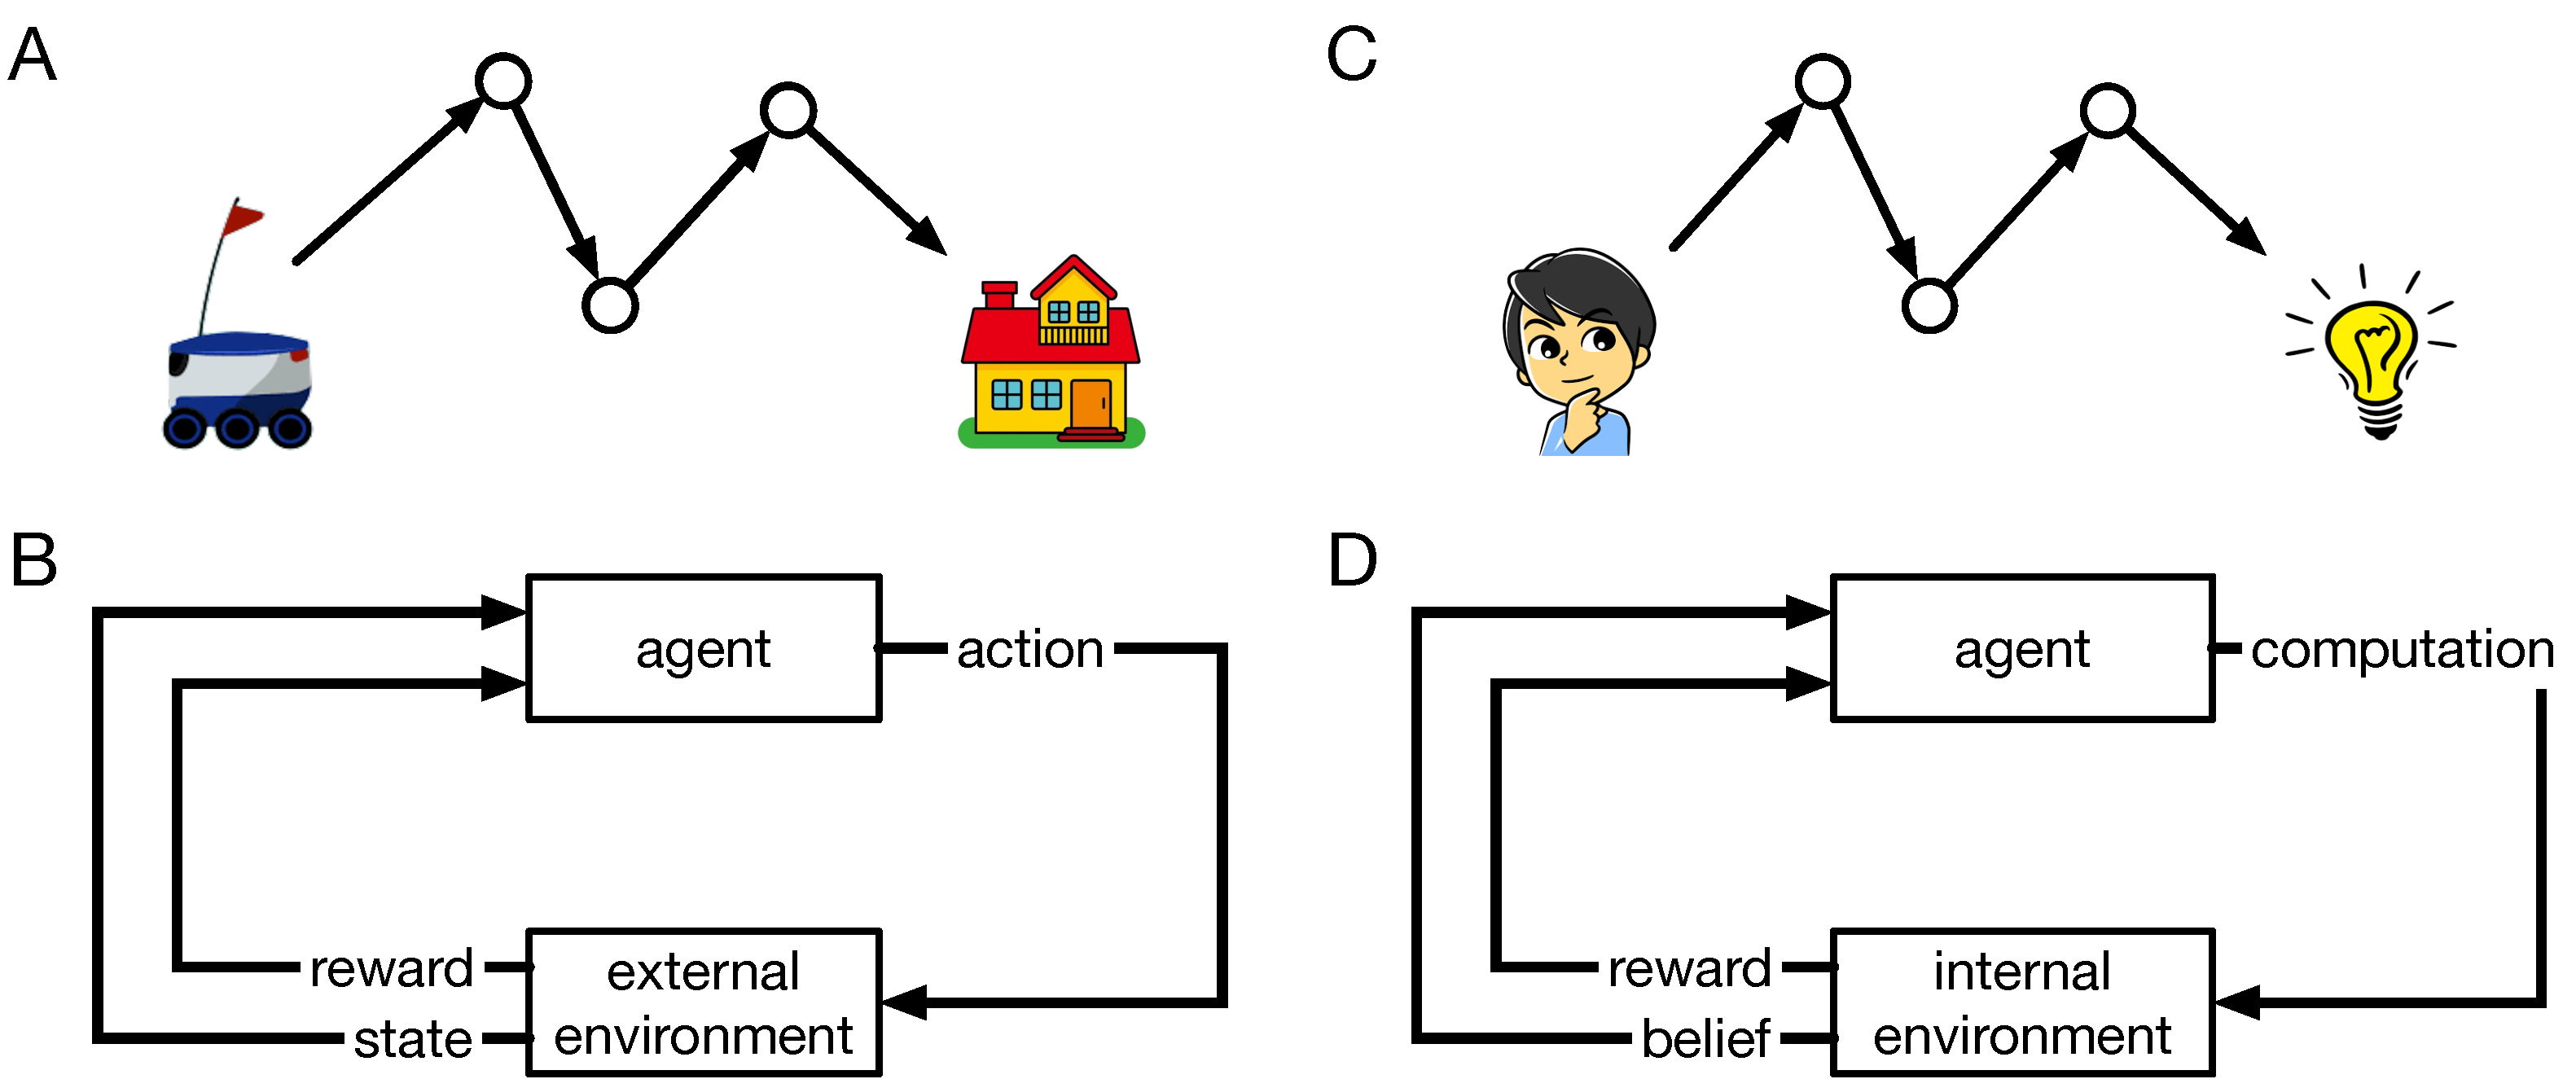
\includegraphics[width=0.9\textwidth]{diagrams/sequential-intuition.pdf}
  \caption{Sequential decision problems posed by external and internal environments.}
  \label{fig:sequential-intuition}
\end{figure}

\figref{fig:sequential-intuition}{c} illustrates a seemingly very different type of situation: a person trying to come up with a solution to a difficult problem. However, as the diagram suggests, the two cases actually share the same basic structure. Both involve an extended interaction between an agent and an environment; but whereas the robot is interacting with an \emph{external} environment, the thinker is interacting with an \emph{internal environment}: their own mind. Just as the robot makes several moves, and visits several locations before reaching the destination, the thinker has several thoughts, and enters several mental states before discovering the solution. Indeed, as illustrated in \figref{fig:sequential-intuition}{d}, this problem can be modeled in precisely the same way as the delivery problem. However, now the actions correspond to computations (thoughts) and the states correspond to beliefs (mental states). Thinking changes one's mental state just as moving changes one's physical state; and it also incurs a cost---at the very least, thinking takes time.

An important property of sequential decision problems is that there is often a dissociation between the short-term reward and the long-term \emph{value} of performing some action. For example, if the robot had the option of simply sitting still, this would incur no cost and would thus be the most rewarding action in a myopic sense. However, the potential for the large reward associated with making a delivery makes paying this cost worthwhile. Thus, moving has value. By the same token, a truly myopic agent (one who only considers immediate rewards) would never do any thinking at all! Thinking only has value insofar as it can inform our future behavior.\footnotemark{}

\footnotetext{Note that, subjectively, thought itself can be rewarding (sometimes intensely so; \citealp{gopnik1998explanation}). However, just as with ``secondary reinforcers'' like money, this is not because thought is inherently valuable, but because it is associated with value. Nevertheless, this association may be deeply engrained, perhaps even genetically so. We return to this question in the conclusion.}

The power of identifying this parallel between external and internal environments is that it allows us to leverage existing knowledge about sequential decision problems (a substantial chunk of AI research) to build rational mechanistic models of cognition. That is, we can apply the same formalisms and algorithms that might help a robot deliver groceries to instead characterize the problem of resource-bounded cognition, and identify cognitive processes that optimally solve that problem.

\section{Optimal and dynamic models of cognition}

The proposed approach builds on a long history of cognitive modeling. In particular, it synthesizes two key features, each of which is prevalent on its own, but which are less commonly seen together: \emph{optimality} and \emph{sequentiality}. These features correspond to assumptions about the nature of cognitive processes. Optimality assumes that the cognitive process maximizes an objective function, and sequentiality assumes that the process can be broken down into a sequence of elementary operations. Neither of these assumptions is likely to be exactly true. But, as previous work has shown, they can both be very useful. In this dissertation, we argue that the intersection of these two features is an especially productive terrain for constructing rational and mechanistic models. But before we further describe that intersection, it is useful to explain each component separately.

% cognition is \emph{dynamic} (sequential, occuring over time), \emph{bounded} (subject to costs or constraints), and \emph{optimized} (maximizing utility). As illustrated in Table~\ref{tab:comparison}, various combinations of these assumptions are made frequently in models of the mind. However, by capturing all three ideas at once, the current approach has advantages that cannot be achieved with any subset.


\subsection{Optimal models}

A cognitive process is optimal if it performs a cognitive function as well as it possibly could. To be precise, an optimal cognitive process is one that produces the maximum value of an \emph{objective function}, out of a set of possible processes:
\begin{equation}\label{eq:intro-optimal}
  π^* = \argmax_{π \in \Pi} U(π).
\end{equation}
Here, $U$ (for utility) is the objective function, and each $\pi \in \Pi$ is a possible cognitive process. Defining an optimal cognitive model thus amounts to specifying the function or goal of the cognitive process (through $U$), and the set of possible processes (through $\Pi$).

Optimality is the defining feature of classic rational models. The prototypical example is statistical decision theory \citep{friedman1948utility}, which states that people should select actions that yield the best outcomes in expectation (i.e., on average). This model is the foundation for neoclassical economics, where it allows analysts to predict aggregate market behavior by assuming that each individual maximizes their own welfare. But it is so abstract that it initially seems to tell us little about cognition itself. Nevertheless, applying the optimization principle in more constrained domains (perhaps implicitly) has yielded important insights about many areas of cognition, including perception \citep{marr1982vision,knill1996perception,najemnik2005optimal} categorization \citep{anderson1991adaptive,ashby1995categorization,tenenbaum2001generalization}, memory \citep{anderson1989human}, and language \citep{goldwater2009bayesian}.

The power of optimization as a tool for cognitive modeling is that it makes decisions for us. That is, it reduces the amount of flexibility we have when specifying a model. This may sound like an impediment---and indeed, it sometimes feels that way---but it can have enormous benefits. Conceptually, optimality is a source of intuition. Cognitive processes can be very complex, and simply observing what people do and trying to reason backwards to how they do it can be challenging---especially if we want to understand \emph{why} they do it that way. Exploring optimal solutions, even when they don't explain human behavior especially well, helps us understand the function of cognitive processes, which in turn helps us generate hypotheses about how those processes actually work.

From a statistical perspective, optimality acts as an inductive bias. Any given behavioral phenomenon is consistent with countless cognitive models \citep{anderson1978arguments}, but only a small subset of those are optimal. If people are well-adapted to their environment, then all else being equal, the optimal models are more likely to resemble the truth than an arbitrary alternative model. Of course, people are not perfectly adapted to their environment; thus, one can always achieve a more accurate model of a particular phenomenon by abandoning the assumption of optimality, which is ultimately false. But when data is limited, or we are exploring a domain we know very little about, or we want to generalize our predictions in non-trivial ways, having a constraint that is \emph{mostly} true can improve our chances of making predictions that are \emph{mostly} accurate.

Problems arise, however, when optimality isn't even mostly accurate. And there are many cases where that seems to be the case. Empirically, Kahneman and Tversky have documented cases where people grossly violate basic laws of logic, probability, and expected utility theory \tocite. But, a simple intuitive example may be even more powerful. Consider playing the game of chess. The optimal move to play in any situation can in principle be defined using basic game theory. One must simply consider all moves one could make, all moves the opponent could make in response, all moves one might make in response to each of those responses.... and so on, until one finds a full sequence of moves that guarantees victory (or at least a draw). But clearly such a strategy is impossible to actually follow.

As famously argued by \citet{simon1955behavioral}, many of the problems people face in the world are like chess, in that computing exactly optimal behavior is practically impossible. Thus, we shouldn't expect people behave optimally---at least not in the classical sense. Does this mean we should abandon the notion of optimality? Perhaps not. According to Simon's notion of \emph{bounded rationality}, we can account for our inability to play perfect chess moves while maintaining the notion of optimality (or at least the slightly less precise notion of rationality) by recognizing that a useful notion of rationality must account for the constraints imposed by our limited computational capacity.

\subsubsection{Accounting for cognitive contraints}

Clearly bounded rationality is a more appropriate benchmark in many cases, but it lacks some of the precision of optimality. To regain that precision while capturing Simon's key insight, we can explicitly formalize the role of cognitive constraints within the optimality paradigm. Specifically, we can define the utility of a cognitive process to account not only for external factors, like the utility of the outcomes of our choices, but also internal factors, like the amount of time and effort we spent making those choices. Formally,
\begin{equation}\label{eq:intro-resource}
  U(\pi) = \E_{a \mid \pi}[U(a)] - \cost(π),
\end{equation}
where $\E_{a \mid \pi}[U(a)]$ is the expected utility of the behavior (or ``action'') the cognitive process produces and $\cost(π)$ captures the cognitive cost associated with executing the cognitive process. This definition of the utility of a cognitive process as an additive combination of behavior-derived utility and cognitive cost is the key defining feature of \emph{resource-rational analysis} \citep{lieder2020resourcerational}.

% One unfortunate consequence of introducing cognitive cost into the objective function is that it creates decisions, precisely the thing we wish to avoid by adopting the optimality assumption. The large space of possible cost functions has been identified as an important challenge for the resource-rational approach \citep{bates2020importance,ma2020multiple}.

For example, in \emph{expected value of control} (EVC) theory, the cognitive process corresponds to a strategy for selecting control signals. In the simplest case, the signal is one-dimensional, with higher values indicating more control. Higher values thus make it more likely 

The cost of the cognitive process, is then the cost of 
\begin{equation}\label{eq:intro-resource}
  U(\pi) = \E_w \left[
    \E_{c \sim π(w)} \left[
      \E_{a \mid c, w} \left[
        U(w, a)
      \right] - \exp(c)
    \right]
  \right],
\end{equation}

Another commonly used cost function is based on information theory. In these models, the cognitive process forms a \emph{representation} of the state of the world, which then informs the action that is taken. The heart of the cognitive process here is the mapping from world states $w$ to mental representations $m$. The utility of this mapping is defined as
\begin{equation}\label{eq:intro-info}
    U(\pi) = \E_w \left[
      \E_{m \sim \pi(w)}[U(w, a_m)]
    \right] - I_\pi(w, m)
\end{equation}
where $a_m$ denotes the action taken given representation $m$, and $I_\pi(w,m)$ denotes the \emph{mututal information} between the state of the world and the representation under the mapping $\pi$. Intuitively, $I$ captures the fidelity of the representation. There are two key ideas to take away from this equation. First, cognitive processes can produce intermediate mental states, which are used to select actions. Second, both the action utility and cost depend on the mental state, and these two forces are in a fundamental conflict. A precise representation of the world allows one to select good actions, but such representations are costly to form.

Information-theoretic models of this sort are commonly used in the study of perception \citep{sims2016rate} and memory \citep{gershman2021rational}, most frequently their intersection. In this literature, the models are typically cast in the language of \emph{rate-distortion theory}. In this context, the utility function captures the discrepancy between the stimulus $w$ and a reconstruction of that stimulus $a_m$ based on the remembered perceptual representation $m$. In a classic application of this approach, \citet{sims2012ideal} show that a model that flexibly allocates informational resource across an arbitrary number of items explains human reconstructions better than a classic model with a fixed number of working memory slots. More recent work showed that people can strategically prioritize more important dimensions of the stimulus (that is, they are sensitive to $U$; \citealp{yoo2018strategic}) and can also allocate more or less resource in total \citep{berg2018resourcerational}. This latter result is interesting because it supports an additive cost like in Equation~\ref{eq:intro-info} over a fixed but costless capacity constraint.\footnote{
  Typically, rate-distortion models are expressed in terms of such a fixed constraint, i.e., maximizing utility subject to a constraint on mutual information. However, because mutual information is an expectation over values of $x$ and $w$, one can find a multiplier on the cost that results in any given average level of expectation (the Lagrange multiplier; see \citealp{ortega2013thermodynamics}).
} Beyond memory, rate-distortion models have also been used to explain the exponential shape of people's generalization curves (\citealp{sims2018efficient}; c.f. \citealp{shepard1987universal} and scalar variability in approximate number representation (\citealp{piantadosi2016rational}, c.f. \citealp{fechner1860elemente}).

In economics, information-theoretic models go under the name \emph{rational inattention}, reflecting the idea that one's mental representation is the result of ignoring features of the world that aren't important to one's decision \citep{sims2003implications,caplin2013behavioral}. This idea was initially developed by \citet{sims1998stickiness} to understand why prices don't respond to changing market conditions as quickly as expected-utility-based models predict. List a few findings... One interesting result from this literature is that, for the commonly used mutual-information cost function, the optimal cognitive process has exactly one representation for each possible action; that is, there is a one-to-one correspondence between $a$ and $m$. This allows one to eliminate $m$ entirely, yielding a reduced form model in which the cost is simply the mutual information between state and action \citep{matejka2015rational}, as proposed in free-energy based models \citep{friston2010freeenergy,ortega2013thermodynamics}. However, while this reduction is mathematically fascinating, it is somewhat unfortunate from a cognitive science perspective. By eliminating the mental representation from the model, we end up with a more sophisticated form of behaviorism, where we attempt to understand a cognitive process simply as a mapping from stimulus to response.

% Importantly, however, this reduction can only be applied under the assumption that all conceivable representational mappings are actually possible. By making stronger, psychologically motivated, assumptions about the form of the cognitive process (the mapping), we can still glean interesting cognitive insights. For example, \citet{bhui2018decision} use 

% \begin{equation}\label{eq:intro-resource}
%   π^* = \argmax_{π \in \Pi} U(\pi) - \cost(π),
% \end{equation}

 % Conceptually $U$ and cost are distinct, referring to external and internal concerns, respectively. However, because both are ultimately a function of the cognitive process, we could just as well include cost within the $U$ function. Thus, at the end of the day, resource-rational models are really optimal models with a specific kind of objective function (and perhaps also a more limited set of possible models $\Pi$).

\subsection{Sequential models}

The fact that cognitive processes are sequential, in the sense that they occur over time rather than all at once, is self-evident. Thus, some notion of sequentiality is an essential feature of a model that captures cognitive mechanisms at any level of detail. Here, however, we will use a slightly more restrictive notion of sequentiality. Specifically, we take sequentiality to mean that cognitive processes can be broken down into a sequences of \emph{elementary information processes} \citep{simon1979information,posner1982information,chase1978elementary}, or simply, cognitive operations.

One widely used class of sequential models are \emph{evidence accumulation} models (also called ``sequential sampling models''), such as the drift diffusion model \citep{ratcliff1978theory}, leaky competing accumulators \citep{usher2001time}, and decision by sampling \citep{stewart2006decision}. According to these models, decision making involves accumulating noisy evidence in favor of each possible choice until the evidence for one choice is sufficiently greater than the evidence for the other(s). That is, the cognitive process can be understood as a sequence of operations, each of which accumulates a small amount of evidence. In their simplest form, there is only one type of operation; these models can explain not only the choices we make (including when we make mistakes), but also how long it takes to make those choices. More complex evidence accumulation models take into account the possibility of attending to different sources of information, such as different options \citep{krajbich2010visual} or attributes \citep{russo1983strategies}; these models can account for (if not predict) additional data such as what we look at when making a decisision, and they can account for systematic deviations from expected utility \citep{busemeyer2019cognitive}.
% For example, these models predict that easier decisions will be made both more consitently and more quickly, and that mistakes will be faster than correct choices.

Another important class of dynamic models, \emph{cognitive architectures}, aims to capture a more diverse range of mental activities, beyond simply accumulating more evidence. Cognitive architectures, most notably ACT-R \citep{anderson1996act} and SOAR \citep{laird1987soar}, explicitly model individual cognitive operations such as perceptually encoding a stimulus, recalling information from memory, and transforming symbolic reprenstations the world. These models can trace their intellectual roots to the infancy of artificial intelligence research \citep{newell1956logic}, where the discovery that digital computers could solve complex problems by breaking them down into a sequence of very simple operations led to the hypothesis that a similar principle might underlie human intelligence \citep{newell1958elements,newell1972human}. 
% The core assumption of these models is that all cognitive processes can be broken down into so-called \emph{elementary information processes} \citep{simon1979information,posner1982information,chase1978elementary}.

Formally, we can define sequentiality as a restriction on the space of possible cognitive processes, $\Pi$. Initially, we might be tempted to say that a cognitive process is simply a sequence of cognitive operations. But this assumes that a given cognitive process will always execute the same sequence of operations, regardless of the state of the world. To account for this dependence, we define each $\pi$ as conditional distribution over cognitive operations given the world state (much as how rate-distortion models define a conditional distribution over representations). Thus, each $\pi \in \Pi$ is defined as
\begin{equation}\label{eq:intro-sequential}
   \pi = P(\cseq \mid w),
\end{equation}
where $\cseq = (c_1, c_2, \ldots, c_n)$ is a sequence of cognitive operations and $P(x)$ denotes a probability distribution over possible values of $x$.

Formalizing dynamic models in this way emphasizes a substantial challenge in constructing them. In principle, any cognitive operation can be executed at any time. Thus, one must not only specify the set of operations and their effects, but also a strategy for how the operations are chosen \citep{payne1988adaptive}. If there are $C$ possible cognitive operations and sequences can go up to length $N$, there are over $C^N$ possible sequences. The space of distributions over those sequences is truly immense. As noted by \citet{howes2009rational}, this space is rarely explored in any kind of systematic manner, which can lead to erroneous conclusions about which cognitive architectures are consistent with a given pattern of behavioral data.

Ecological rationality goes here.

% Constructing dynamic models poses a substantial challenge, however, particularly when there are many different elementary operations. Because any number of cognitive operations can be executed at any time, one must not only specify the set of operations and their effects, but also a strategy for how the operations are chosen \citep{payne1988adaptive}. In practice this is often done in an ad hoc manner (c.f., \citealp{howes2009rational}).

% \begin{equation}
%   \cost(π) = \expect{\sum_t \cost(c_t)}{c_t \sim π}
% \end{equation}


\subsection{Optimal sequential models}

Having defined and briefly reviewed optimal and dynamic models, we now turn to the key question: how can we combine these ideas? Like the optimal models, we assume that the cognitive process people use maximizes a utility function, specifically one that takes into account both the utility of our actions and the cost of the process. And like sequential models, we assume that cognitive processes correspond to distributions over sequences of cognitive operations. This results in 
\begin{equation}
  π^* = \argmax_{π} \E_w \left[
   \E_{\cseq \sim \pi(w)} \left[
      U(w, a_n) - \sum_i \cost(c_i)
    \right]
  \right]
\end{equation}
where $a_n$ (I think I want $m$ in here...)


% \begin{equation}
%     π^* = \argmax_{\cseq}\,  U(\cseq) - \cost(\cseq).
% \end{equation}


% \begin{equation}
%   π^* = \argmax_{π} \E_{\cseq \mid \pi} \left[
%     U(a_n) - \sum_i \cost(c_i)
%   \right]
% \end{equation}
% \begin{equation}
%   π^* = \argmax_{π} \E_{\cseq \mid \pi} \left[
%     \E_{a \mid \cseq} [ U(a) ] - \sum_i \cost(c_i)
%   \right]
% \end{equation}

% This substitution yields little insight on its own. Specifically, what is the utility of a sequence of cognitive operations? Intuitively, the utility of cognition comes from how it affects our actions. Thus, let $\mathrm{act}_N$ be the action we would take after executing the cognitive process $(c_1, c_2, \ldots c_N)$. Further, we can assume that the cost of each operation is independent. This yields
% \begin{equation}
%     π^* = \argmax_{(c_1, c_2, \ldots c_N)} U(\mathrm{act}_N) - \sum_i^N \cost(c_i).
% \end{equation}
% That is, an optimal sequential cognitive process is one which maximizes the utility of the action that the cognitive process produces minus the total cost of all the operations it performs. We express this intuition more precisely in the following chapter (Equation~\ref{eq:optimal-meta-policy-expanded}).

% problem: this isn't actually sequentially optimal


% \section{Alternative approaches for rational mechanistic modeling}

% Having defined and briefly reviewed optimal and dynamic models, we now turn to the main question explored by this disseration. How can we construct rational mechanistic models? The answer proposed here is the construction of optimal sequential models. But before

% This is by no means a new question, nor is this dissertation the first to propose a general framework for constructing such models. In the following sections, we briefly review this past work, with an emphasis on ...

% \subsection{Ecological rationality}





% \subsection{Optimal but not dynamic}




% In this way, resource-rationality is more similar \emph{ecological rationality}, a framework based on the idea that people use computationally frugal heuristics, which are highly effective for the kinds of problem that people actually encounter \citep{gigerenzer1999simple,goldstein2002models,todd2012ecological}. For example, if the other players in an environment are using a wide variety of decision strategies, then a heuristic that ignores the other players payoffs entirely may perform best \citep{spiliopoulos2020map}. However, while proponents of ecological rationality explicitly reject the notion of optimization under constraints (e.g. \citealp{gigerenzer1999simple}, Ch. 1), optimization is at the heart of resource-rational models.



% More recently, the notion of optimality has been extended to account not only for the demands imposed by the external environment but also the demands imposed by our own cognitive limitations \citep{howes2009rational,lewis2014computational,gershman2015computational,griffiths2015rational,lieder2020resourcerational}. This approach dates back to Simon \citep{simon1955behavioral} and has been especially useful in the domain of decision-making, where it has been used to explain both how long people deliberate \citep{bogacz2006physics,drugowitsch2012cost,tajima2016optimal,tajima2019optimal,fudenberg2018speed} and also what people think about \citep{callaway2021fixation,jang2021optimal} while making ``simple'' (i.e., non-sequential) choices. However, to the best of our knowledge, there has been no such analysis in the domain of planning, despite the especially critical role that computational limitations play in this case (but c.f. \citep{sezener2019optimizing,mattar2018prioritized} for closely related efforts, which we discuss further below).



% The use of optimization in cognitive models is more controversial. 


% The basic premise of the approach is that the mind should be well adapted to its environment, through some combination of learning and evolution \citep{anderson1990adaptive}. Optimization simply takes this idea to the logical extreme, assuming that the mind is adapted \emph{as well as possible} to the environment.



% % Dynamic: DDMs.

% % Control: attention, metacognition.

% % Adaptive: rational analysis, economics

% % More interesting are models that capture two of the three properties.

% % Dynamic + Control: cognitive architectures.

% % Dynamic + Adaptive: ???

% % Control + Adaptive: EVC


% % \newcommand{\yes}{\checkmark &}
% % \begin{table}[tb]
% %   \caption{Classification of cognitive models.}
% %   \label{tab:comparison}
% %   \centering
% %   \begin{tabular}{cccc|c}\toprule
% %   Dynamic & Controlled & Optimized & Notable Examples \\
% %   \midrule
% %   \yes & &
% %     DDM 
% %   \\ & \yes &
% %     Attention, metacognition 
% %   \\ & & \yes
% %     Rational analysis, economics 
% %   \\ \yes \yes &
% %     Cogntive architectures, ecological rationality
% %   \\ \yes & \yes 
% %     Bogacz ?
% %   \\ & \yes \yes 
% %     EVC, information-theoretic
% %   \\ \yes \yes \yes
% %     This dissertation 
% %   \\ \bottomrule
% %   \end{tabular}
% % \end{table}


% sampling
% information theoretic
% rational analysis
% ecological rationality
% EVC
% cognitive architectures

% % \begin{table}[tb]
% %   \caption{caption here}
% %   \label{tab:tablename}
% %   \centering
% %   \begin{tabular}{ccc|c}\toprule
% %   Dynamic & Control & Adaptive & Examples \\
% %   \midrule
% %   \yes & &     DDM \\
% %   & \yes &     Attention, metacognition \\
% %   & & \yes     Rational analysis, economics \\
% %   \yes \yes &  Cogntive architectures \\
% %   \yes & \yes  ? \\
% %   & \yes \yes  EVC \\
% %   \yes \yes \yes  This dissertation \\
% %   \bottomrule
% %   \end{tabular}
% % \end{table}



% In comparison to non-rational dynamic models, the proposed approach
% - naturally captures metacognition and control
%   - c.f. aDDM which assumes random attention
%   - c.f. metamemory which ignores control
% - avoids combinatorial search

% Compared with non-sequential rational models, 



%  % the problem posed by the internal environment (what I will call the \emph{meta-level} problem) is exactly analagous to the problem posed by the external environment (the \emph{object-level} problem). 








% In comparison to non-dynamic rational models
% - captures the process/mechanism (c.f. information-theoretic accounts)
% - more optimal
% - captures sequential dependence



% % Taken from planning (cut there?)
% These challenges---hypothesis generation, generalizable prediction, and functional explanation---are not unique to planning; indeed, they arise in nearly all areas of cognition. In many domains, progress in addressing these challenges has been made by analyzing optimal solutions to the problem a cognitive system is meant to solve \citep{marr1982vision,anderson1990adaptive}. This approach has generated insight into a wide range of problems, including decision-making \citep{savage1954foundations}, generalization \citep{tenenbaum2001generalization}, categorization \citep{anderson1991adaptive,ashby1995categorization}, perception \citep{knill1996perception}, and information-seeking \citep{oaksford1994rational,gureckis2012selfdirected}. More recently, the notion of optimality has been extended to account not only for the demands imposed by the external environment but also the demands imposed by our own cognitive limitations \citep{howes2009rational,lewis2014computational,gershman2015computational,griffiths2015rational,lieder2020resourcerational}. This approach dates back to Simon \citep{simon1955behavioral} and has been especially useful in the domain of decision-making, where it has been used to explain both how long people deliberate \citep{bogacz2006physics,drugowitsch2012cost,tajima2016optimal,tajima2019optimal,fudenberg2018speed} and also what people think about \citep{callaway2021fixation,jang2021optimal} while making ``simple'' (i.e., non-sequential) choices. However, to the best of our knowledge, there has been no such analysis in the domain of planning, despite the especially critical role that computational limitations play in this case (but c.f. \citep{sezener2019optimizing,mattar2018prioritized} for closely related efforts, which we discuss further below).
